%!TEX root = ../thesis.tex
\chapter{Introduction}
\label{chap:introduction}

The majority of the stars are born together. \citet{2000AJ....120.3139C} reports that $50-70\%$ of very young, $\leq10$ \gls{myr}, and $25-70\%$ of the young, $\leq100$ \gls{myr}, stellar populations are formed in groups. \citet{2003AJ....126.1916P} and \citet{2003ARA&A..41...57L} find that among 80\% to 90\% of the stars are formed in groups with more than 100 members, which are called star clusters. Furthermore, as indicated by the former authors, these populous clusters represent 22\% of the regions where stars form. The remaining of the star forming regions are small associations, with 5 to 30 members, where only up to 10\% of the stars are formed. However, only less than 7\% of these populous clusters survives as gravitationally bounded clusters when reaching an age of a few hundred \gls{myr} \citep{2003ARA&A..41...57L}. The remaining 93\% of the star forming regions will become unbound and their stars will freely populate the galaxy. Thus, to understand the general rules that govern how the majority of stars forms, as well as the properties of the stars that populate our galaxy, it is crucial to fully decode the formation and early evolution of stellar clusters. 

Astrophysicists, like archeologists and palaeontologists, can not willingly reproduce the vast majority of their studied phenomena. Although some experiments can be performed in specific situations (e.g. the chemical and physical  properties of dust and gas), astrophysics remains an observational science. For this reason, to test the validity of their hypotheses, astrophysicists rely on statistical studies carried out over carefully designed observations. In particular, the understanding of the star formation process requires carefully designed observations of  stellar clusters whose ages cover the early stages of their evolution.

The objective of this work is the construction, test and validation of a statistical tool, an intelligent system specifically, that given the carefully designed data of a stellar cluster, recovers the statistical distributions of its populations. In particular, it should deliver the cluster luminosity distribution, which can be transformed into the mass distribution given an evolutionary model and the cluster age. The mass distribution is a fundamental product of the star formation process. It contains the fingerprints of the early phases of star formation and subsequent cluster evolution.

An homogeneous and precise mass distribution inventory for clusters of diverse ages and forming environments will allow the astrophysical community to test the current theories of the star formation process. In particular, it will allow to solve the questions about universality of the \gls{imf} (see next Section) and the role played by the physical properties of the cluster environment.    

The remaining of this Chapter is structured as follows. In Section \ref{sect:IMF}, I describe the importance of the initial mass distribution and some of its current models. In Section \ref{sect:numerical_simulations}, I report the current status of numerical simulations of cluster formation and its impact on the understanding of the star formation process. In Section \ref{sect:DANCeproject}, I describe the project \gls{dance}, its objectives and its carefully designed observations of stellar clusters. This work is part of that project and makes use of its observations. In Section \ref{sect:current_methodologies}, I comment on the past and current methodologies to select members of clusters and associations. Finally in Section \ref{sect:newIS}, I briefly describe the methodology adopted for this new statistical tool, and its advantages over the previous works. 

\section{The initial mass function of stellar clusters}
\label{sect:IMF}

In his seminal work \citep{Salpeter1955}, Edwin Salpeter defined the \emph{original mass function}, $\xi(M)$, as

\begin{equation}
\mathrm{d}N= \xi(M)\mathrm{d}(\log_{10} M) \frac{\mathrm{d}t}{T_0},\nonumber
\end{equation}
where $\mathrm{d}N$ is the number of stars in the mass range $\mathrm{d}M$ created in the time interval $\mathrm{d}t$ per cubic parsec, and $T_0$ is the age of the galaxy. Following \citet{Chabrier2003b},  the \gls{mf} at the observed time $t$, is

\begin{equation}
\xi(\log_{10} M)=\frac{\mathrm{d}N}{\mathrm{d}(\log_{10} M)},\nonumber
\end{equation}

where $N$ is the stellar number density, and $M$ the mass. The \gls{imf} is defined as the \gls{mf} at the time of stellar formation $t=t_0$. The logarithmic transformation of the mass,
\begin{equation}
\xi(M)=\frac{1}{M \ln 10} \xi (\log_{10} M),\nonumber
\end{equation}
is convenient due to the large range of masses covered by the star formation process.

Notice that neither the \gls{imf} nor the \gls{mf} are probability \glspl{pdf} of the mass (see Section \ref{sect:introprobability} for the definition of a \gls{pdf}). Nevertheless, they can be transformed into \glspl{pdf} by a normalisation constant, which can be computed by integrating them as functions of the mass over the mass domain. In this work, I will use the \gls{md} in the logarithmic scale, denoted by $\xi_L (\log_{10}M)$, as a proxy for the \gls{mf}. Thus,

\begin{equation}
\xi_L (\log_{10} M) \propto \xi (\log_{10} M).\nonumber
\end{equation}

The measuring and understanding of the \gls{imf} is a central topic in the study of star formation. It is also essential in other areas of astrophysics, from planetary formation, where it appears that the mass of the host star plays an important role in the formation of the planetary system \cite[see for example][]{2015ApJ...814..130M}, to galactic evolution \citep{1998ASPC..142....1K} and cosmology \cite[see for example][]{2012MNRAS.423.3601N}. 

The theories that predict the origin of the \gls{imf} can be categorised into deterministic and stochastic \citep{Offner2014}. The former postulate that stellar masses are deterministically inherited from the initial core masses via accretion from the gas reservoir of the parent molecular cloud. Thus, the \gls{imf} can be directly mapped from the distribution of initial core masses, and the understanding of the former reduces to that of the latter. On the other hand, stochastic models postulate that the stellar masses are independent of the initial core masses. Among these models, there are those proposing that stellar masses are determined by dynamical interactions and competitive accretion. For more details see \citet{Offner2014} and references therein. 

  The observational studies of the \gls{imf} are conditioned on the ages of the stellar populations under analysis (their \gls{mf} at their corresponding ages), and rely deeply on the assumed processes that link the observed present-day \gls{mf} to the \gls{imf}. While the resulting models for the \gls{imf} are analytical functions of the mass, the observed \gls{mf} are commonly expressed with points, histograms or \glspl{kde}\footnote{\glspl{kde} are non-parametric ways to estimate a probability density function by means of an independently and identically distributed sample drawn from it.}.

The most common forms to describe the \gls{imf} are the power-law functions of Salpeter \citep{Salpeter1955}, Miller and Scalo \citep{1979ApJS...41..513M}, and Kroupa \citep{2001MNRAS.322..231K,2002Sci...295...82K,2013pss5.book..115K,Thies2007,2008MNRAS.390.1200T}, and the log-normal functions of Chabrier \citep{Chabrier2003a,Chabrier2003b,Chabrier2005}. Other functional forms include the truncated exponential \citep{2001AGM....18S0551D}, the Pareto-Levy family distribution \citep{2012MNRAS.423.1018C}, and a log-normal with power-laws at high and low mass ranges \citep{2013MNRAS.429.1725M}. For the sake of simplicity, I will only explain the classical ones of Salpeter, Chabrier, and Kroupa.

\citet{Salpeter1955} derived his famous \gls{imf} using a luminosity function resulting from the compilation of the works of \citet{1939POMin...7....1L,1941NYASA..42..201L} and \citet{1925PGro...38D...1V,1936PGro...47....1V}. Then, he transformed it into a \gls{mf} using a mass-luminosity relation that he obtained after adopting a series of masses and luminosities from the literature. His \gls{mf} has the form

\begin{equation}
\xi(M)=0.03 \left(\frac{M}{M_{\odot}}\right)^{-1.35},\nonumber
\end{equation}
with $M$ in the range $0.3\,M_{\odot}$ to  $17\,M_{\odot}$. Its units are $ M_{\odot}^{-1} \cdot pc^{-3}$.

\citet{Chabrier2003a,Chabrier2003b} derived his \gls{pdmf} from the nearby luminosity functions of both the $V$ band \citep{1986AJ.....91..621D} and the $K$ band \citep{1990ApJ...350..334H} for the solar neighbourhood ($\leq$5 pc). He used the \citet{2000A&A...364..217D} and \citet{1998A&A...337..403B} mass-magnitude relations in $V$ and $K$ bands, respectively, to transform the luminosity functions into masses. Then, he fitted a log-normal form to the single objects with masses below 1 $M_{\odot}$. The \gls{pdmf} he found, in units of $(\log M_{\odot})^{-1}\cdot pc^{-3}$, is 

\begin{equation}
\xi(\log m)_{m\leq1M_{\odot}}=0.158_{-0.046}^{+0.051} \times \exp{\left\{-\frac{(\log m - \log 0.079_{-0.016}^{+0.021})^2}{2 \times (0.69_{-0.01}^{+0.05})^2}\right\}}.\nonumber
\end{equation}

As shown by \citet{1986FCPh...11....1S}, 1 $M_{\odot}$ is the limit at which the \gls{pdmf} starts to differ from the \gls{imf}. Therefore, \citet{Chabrier2003b} uses his \gls{pdmf} as the \gls{imf} below the 1 $M_{\odot}$ limit. Above it, he adopts the Salpeter \gls{imf},

\begin{equation}
\xi(\log m)_{m>1M_{\odot}}= 4.43\times10^{-2}\cdot m^{-1.3\pm0.3}.\nonumber
\end{equation}

As shown by \citet{1991MNRAS.251..293K}, the discrepancies between the luminosity functions derived from photographic samples and from trigonometric parallaxes of nearby stars can be accounted with unresolved binaries. For this reason, \citet{Chabrier2003a} derived the \gls{pdsmf} for unresolved systems. It takes into account each object as a possible unresolved binary or system. This \gls{pdsmf} has the form,

\begin{equation}
\xi(\log m)_{m\leq1M_{\odot}}=0.086\times \exp{\left\{-\frac{(\log m - \log 0.22)^2}{2 \times (0.57)^2}\right\}},\nonumber
\end{equation}
with the same normalisation and coefficients of the \gls{imf} above 1 $M_{\odot}$.

Later, \citet{Chabrier2005} included in his analysis the revision that \citet{2002AJ....124.2721R} made to the sample of \citep{1986AJ.....91..621D}, and the extended sample of 8 pc from \citet{2004AJ....128..463R}. His new \gls{pdmf} is

 \begin{align}
\xi(\log m)_{m\leq1M_{\odot}}=&0.093\times \exp{\left\{-\frac{(\log m - \log 0.2)^2}{2 \times (0.55)^2}\right\}},\nonumber\\
\xi(\log m)_{m>1M_{\odot}}=& 0.041\times m^{-1.3\pm0.3}.\nonumber
\end{align}

And his new \gls{pdsmf} is
 \begin{align}
\xi(\log m)_{m\leq1M_{\odot}}=&0.076\times \exp{\left\{-\frac{(\log m - \log 0.25)^2}{2 \times (0.55)^2}\right\}},\nonumber\\
\xi(\log m)_{m>1M_{\odot}}=& 0.041\times m^{-1.3\pm0.3}.
\end{align}

The canonical \gls{imf} of Kroupa \citep{2013pss5.book..115K} is a three-segment power-law, with two segments describing the \gls{imf} of the stars, while the third does it for \gls{bd}\footnote{Brown-dwarfs are substellar objects with masses in the range from 10 to 80 Jupiter masses (0.01$M_{\odot}$ to 0.075 $M_{\odot}$). Because there is no fusion of hydrogen in their cores, these objects are not classified as stars.}. It has the following analytical representation

\begin{equation}
\label{eq:KroupaBD}
\xi_{BD}(m)=\frac{k}{3}\cdot\left(\frac{m}{0.07}\right)^{-0.3\pm0.4}, \hspace{3.5cm} 0.01M_{\odot} < m \leq 0.15 M_{\odot},
\end{equation}
\begin{align}
\label{eq:KroupaStars}
\xi(m)=& k\cdot \left(\frac{m}{0.07}\right)^{-1.3\pm0.3}, \hspace{3.5cm} 0.07M_{\odot} < m \leq 0.5 M_{\odot},\nonumber\\
\xi(m)=& k\cdot \left(\frac{0.5}{0.07}\right)^{-1.3\pm0.3}\cdot  \left(\frac{m}{0.5}\right)^{-2.3\pm0.36}, \ \ \ \ 0.5 M_{\odot} < m \leq 150 M_{\odot},
\end{align}
where $k$ is a constant.
 
 \citet{Thies2007} explored the parametric space of the  \gls{imf} for the \gls{bd} population. They performed a $\chi^2$ fit of the maximum \gls{bd} mass ($m_{max,BD}$), the slope of the \gls{bd} \gls{imf} ($\alpha_{BD}$ in Eq. \ref{eq:KroupaBD}), and the population ratio ($\mathcal{R}_{pop}$), which is the ratio of individual \gls{bd} to individual stars. They performed this fit on literature data from the Trapezium, Taurus, IC 348 and the Pleiades nearby clusters. Figure \ref{fig:IMFThies2007}, which reproduces their Figure 7, shows their results in these four clusters. In their work, the stellar \gls{imf} is the canonical one (Eq. \ref{eq:KroupaStars}). In the case of the Pleiades and IC 348, the slope of the \gls{bd} \gls{imf} remained the canonical value $\alpha_{BD}=0.3$ due to the sparse data, and the Pleiades  incomplete data particularly. The resulting system \gls{imf} is also shown as the solid curve. It results from the addition of the two \glspl{imf} (\gls{bd} and stars) but without an overlap or discontinuity between them \cite[see][for details]{Thies2007}.
 
 \begin{figure}[htbp]
\begin{center}
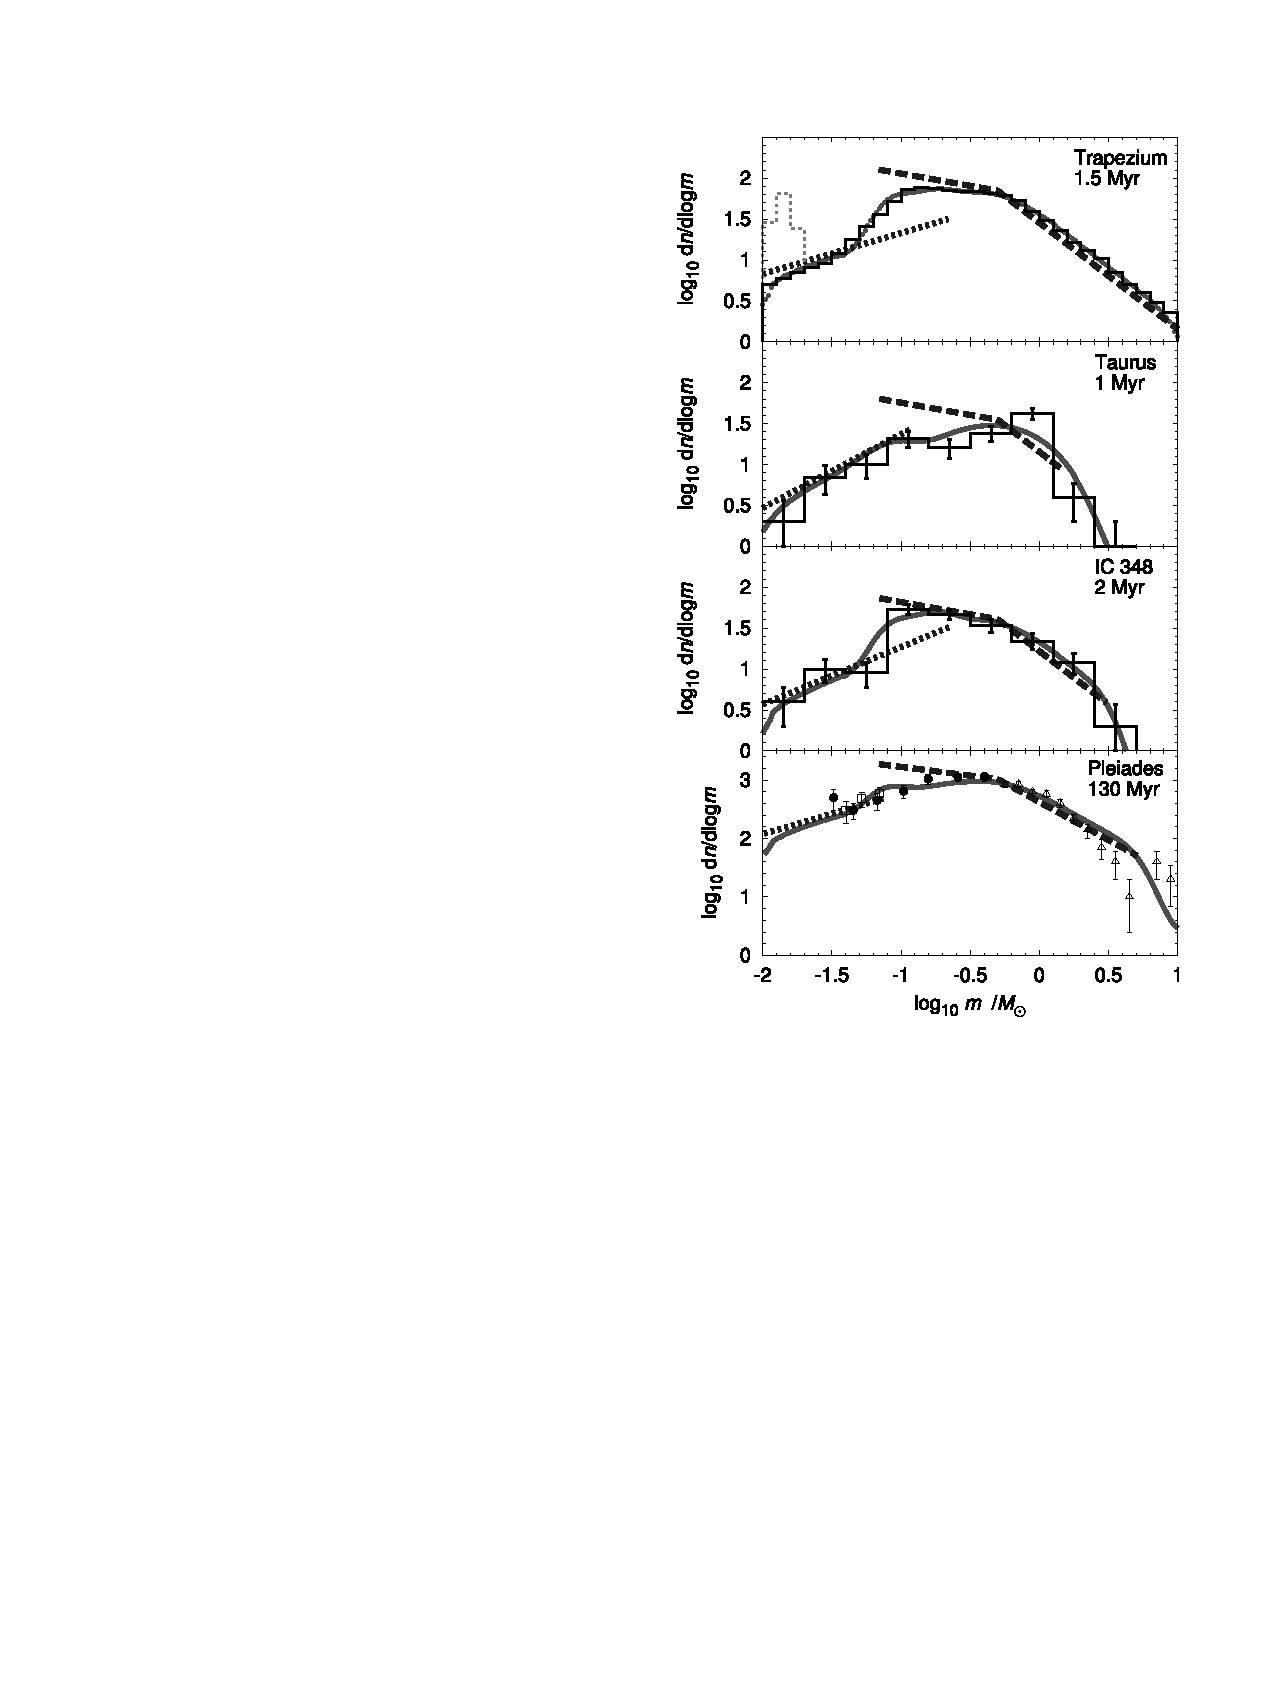
\includegraphics[width=0.8\textwidth]{background/Figures/F7_Thies2007.pdf}
\caption{Observed mass distribution (histograms and dots) of the Trapezium, Taurus, IC348 and the Pleiades nearby clusters (from top to bottom). Also shown are the canonical stellar (long dashed line), fitted \gls{bd} (dotted), and system (solid curve) \glspl{imf} of \citet{Thies2007} . Reproduced from Figure 7 of \citet{Thies2007}, \textit{\usebibentry{Thies2007}{Title}}, \usebibentry{Thies2007}{Journal}, Vol. \usebibentry{Thies2007}{Volume}}
\label{fig:IMFThies2007}
\end{center}
\end{figure}
 
As shown in this Section, the \gls{imf} has been the subject of several studies which have transformed our knowledge about it. This knowledge evolved from the simple and efficient model of \citet{Salpeter1955} in the high mass range, to the more complicated and still controversial models of \citet{Thies2007, 2013pss5.book..115K} for the \gls{bd} and low-mass stars. In the literature, the \gls{imf} of Chabrier \citep{Chabrier2003a,Chabrier2003b,Chabrier2005} is often the preferred one. Although these models currently explain many of the observed phenomena, our knowledge of the physical processes that lead to the observed \gls{imf} is still incomplete. In an attempt to address the latter, the numerical simulations of the star formation process have done great progress. The next section is a tiny review of what these simulations have achieved in the past years.


\section{Numerical simulations of the early stages of star formation}
\label{sect:numerical_simulations}

In the first decade of this century, numerical simulations of star forming regions have proven to be of paramount importance in decoding the very early stages of the star formation process \cite[e.g][]{2003MNRAS.339..577B,2005A&A...435..611J,2009MNRAS.392..590B,2009MNRAS.392.1363B,2009MNRAS.397..232B}. For example, \citet{2003MNRAS.339..577B} using smooth particle hydrodynamics were able to simulate the collapse and fragmentation of a large-scale ($50\,M_{\odot}$ within 0.375 pc radius) turbulent molecular cloud to form a stellar cluster. During the very first 0.1 \gls{myr}, which was the time covered by their simulation, they were able to simultaneously form discs and binary stars. The cloud formed roughly equal numbers of stars and \gls{bd} (23 and 27, respectively) resulting in a mass distribution with a flat slope in the range $0.01-0.5 M_{\odot}$ (see Fig. \ref{fig:IMFBate2003}). \citet{Offner2014} provides a review of the stellar initial mass distribution, and of the physical effects included in numerical simulations (radiative feedback, competitive accretion, dynamical interactions, magnetic fields) particularly. 

In recent years, the works of \citet{2015ApJ...815...27K} and \citet{2015MNRAS.452..566B}, using the cold collapse paradigm (neglecting magnetic fields, radiative transfer and feedback), were able to probe that the main source driving the star formation process is gravity. Their simulations were typically run until 0.85 \gls{myr} in a box of 3 pc of side, and with masses in the few thousands of $M_{\odot}$. The mass distribution obtained by \citet{2015ApJ...815...27K} reproduces reasonably well the current models of the initial mass distribution. In particular, the \gls{imf} of \citet{Chabrier2005} down to  $0.1\,M_{\odot}$ (see Fig. \ref{fig:IMFKuznetsova}). However, they produce too few low-mass stars and brown dwarfs.

% Remaining issues

Numerical simulations are of great use in the understanding of the star formation process, in the very early phases ( $\leq$1 \gls{myr}) of its evolution particularly.  Despite the fact that many of these simulations are in agreement with the observed mass distributions, currently they i) do not incorporate all astrophysical effects, ii) resolve close binaries and multiple systems, and iii) produce enough stellar objects to improve the statistics \citep{Offner2014}. Furthermore, these simulations require input from the observations (e.g. density, turbulence and magnetic fields in the molecular cloud). More importantly, they require feedback from the observations in order to fine tune the parameters of the physical processes. Real and simulated data must be compared in order to improve the latter. Thus, to constrain the current theories of the star formation process, precise and detailed studies of the early phases of cluster formations are still required. This is the objective of the \gls{dance} project, from which the present work is part of.


% Why are these issues important?
\begin{figure}[ht!]
\begin{center}
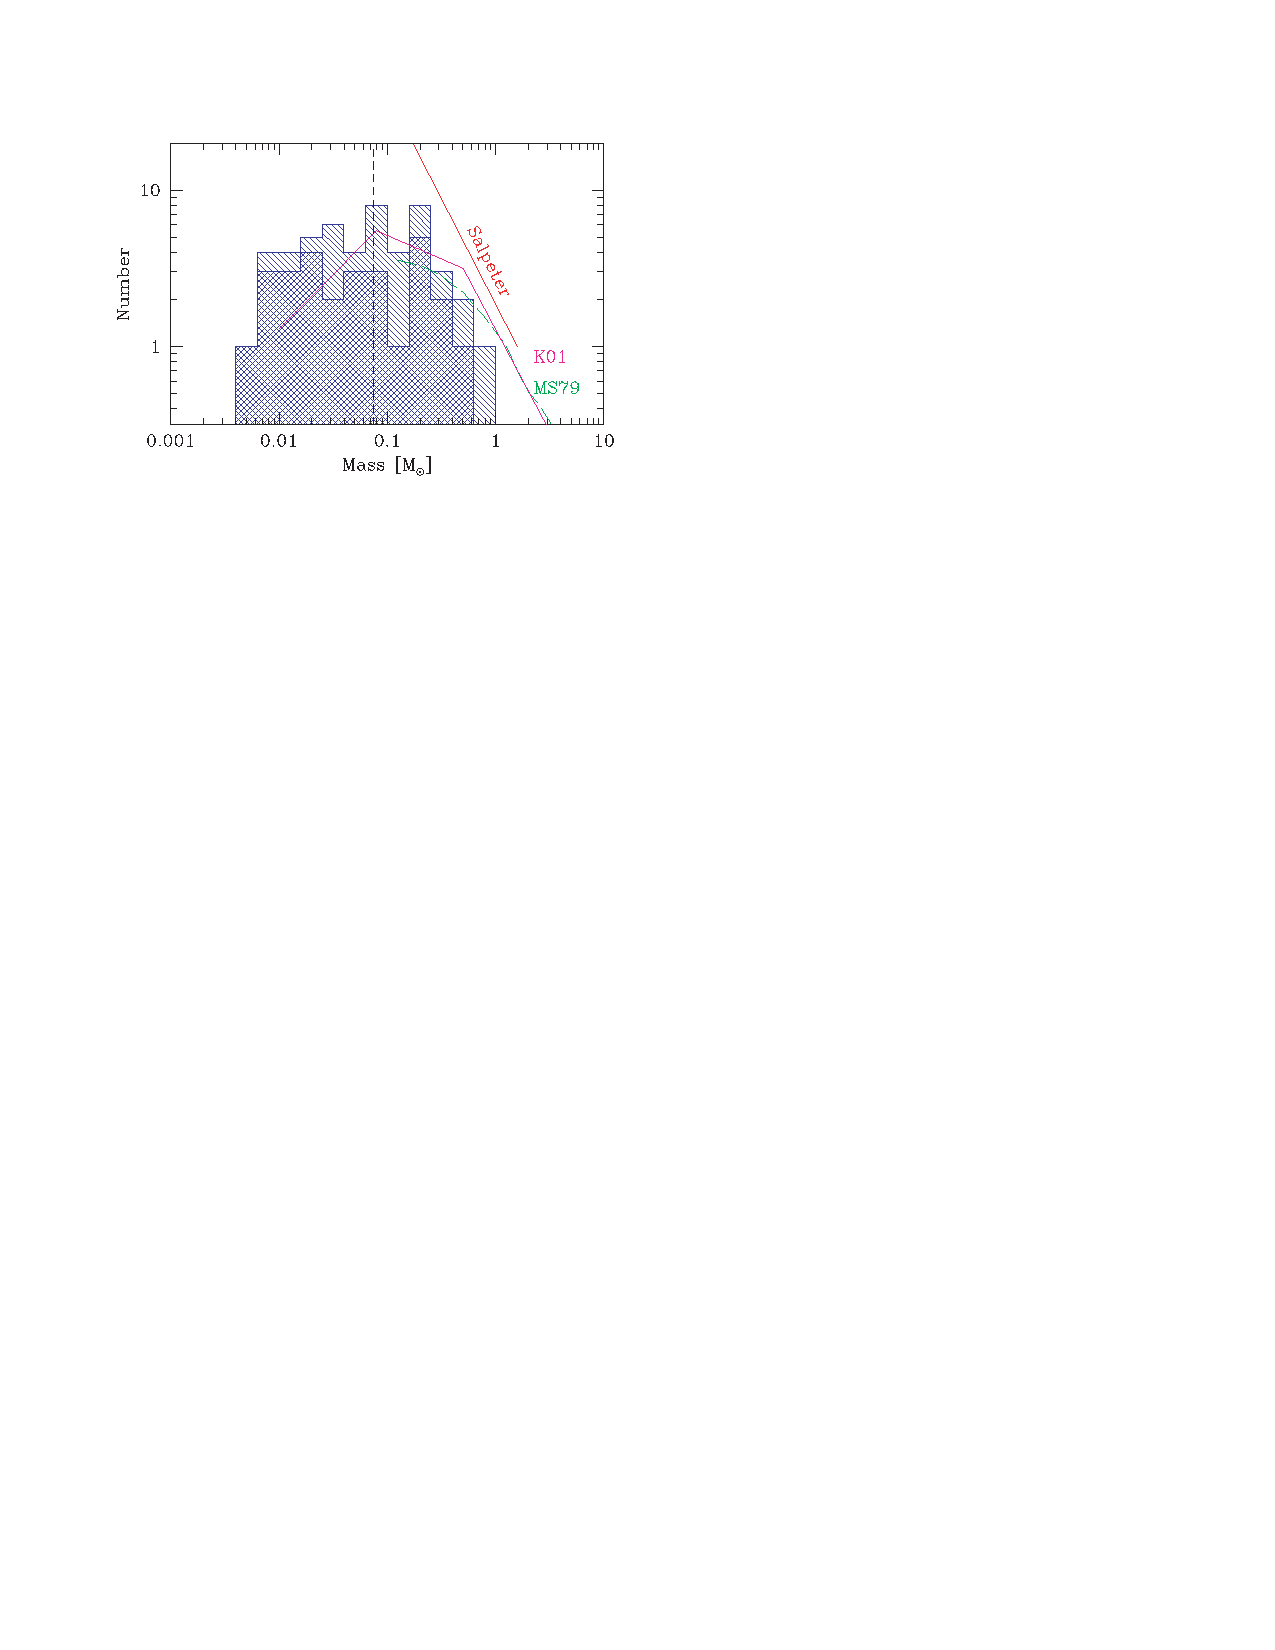
\includegraphics[width=0.8\textwidth]{background/Figures/F10_Bate2003.pdf}
\caption{Mass distribution resulting from the numerical simulation of \citet{2003MNRAS.339..577B}. The lines show the mass distributions of \citet{Salpeter1955}, \citet{1979ApJS...41..513M} and \citet{2001MNRAS.322..231K}. Reproduced from Figure 10 of \citet{2003MNRAS.339..577B}, \textit{\usebibentry{2003MNRAS.339..577B}{Title}}, \usebibentry{2003MNRAS.339..577B}{Journal}, Vol. \usebibentry{2003MNRAS.339..577B}{Volume}}
\label{fig:IMFBate2003}
\end{center}
\end{figure}

\begin{figure}[ht!]
\begin{center}
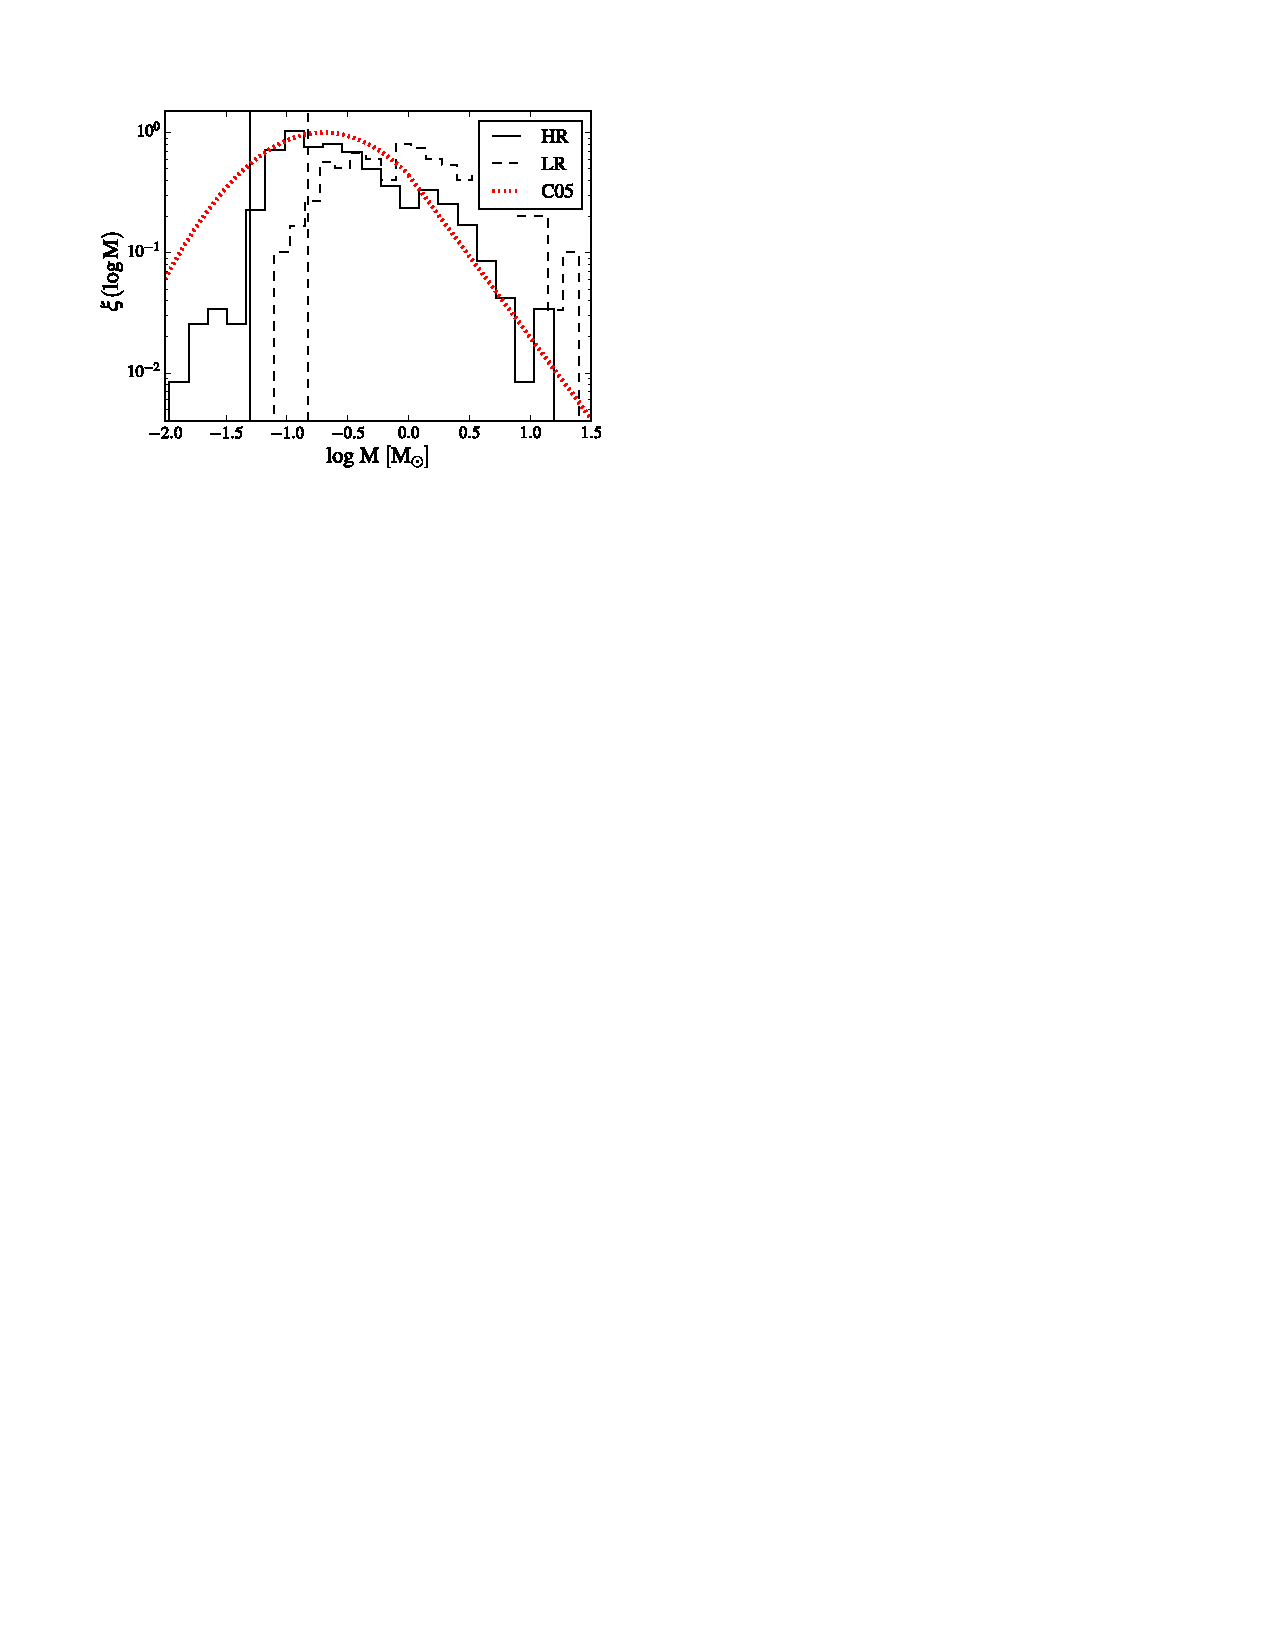
\includegraphics[width=0.8\textwidth]{background/Figures/F11_Kuznetsova2015.pdf}
\caption{Mass distribution resulting from the numerical simulation of \citet{2015ApJ...815...27K}. The High (solid line) and Low (dashed line) resolution simulations reach $0.05\, M_{\odot}$(solid vertical line) and $0.15\, M_{\odot}$ (dashed vertical line), respectively. Also shown the normalised \gls{imf} of \citet{Chabrier2005} (red dashed line). Reproduced from Figure 11 of \citet{2015ApJ...815...27K}, \textit{\usebibentry{2015ApJ...815...27K}{Title}}, \usebibentry{2015ApJ...815...27K}{Journal}, Vol. \usebibentry{2015ApJ...815...27K}{Volume}}
\label{fig:IMFKuznetsova}
\end{center}
\end{figure}

\section{The DANCe project}
\label{sect:DANCeproject}

The \gls{dance}\footnote{\url{http://project-dance.com}} project is an international and multidisciplinary collaboration of researchers whose main objective is \textsl{unravelling the origin of the mass function} of stellar \glspl{nyc}. This objective demands a thorough compilation of resolved star forming populations over the entire mass spectrum and in diverse star forming environments. It requires complete catalogues of the star cluster members, and only those members. Disentangling star cluster members from the field population is a titanic task that the astrophysical community is on the verge of completing thanks to the future \emph{Gaia} \citep{GAIA} data. However, even with Gaia, the development and success of star formation theories will be pending a comprehensive identification of the sub-stellar populations and the internal dynamics of embedded cluster cores. \emph{Gaia} will leave aside the most massive \gls{bd} and planets, reaching only down to 0.03 $M_{\odot}$ on the best cases \citep{Sarro2013}. Furthermore, \emph{Gaia} reaches the 20 mag limit in the $G$ band \cite[350 nm to 1000 nm][]{2010A&A...523A..48J} what makes it almost blind to the dust and gas in which the majority of the star forming regions are still embedded. 

The \gls{dance} photometric and astrometric measurements will complement \emph{Gaia}'s exquisite astrometric precision in a selected list of star forming regions, which is shown in Table \ref{tab:maintargets}. In addition, its secondary targets are also listed in Table \ref{tab:secondarytargets}. A pilot study of the \gls{dance} data properties has already been conducted on the Pleiades cluster. For more details on it I refer the reader to Section \ref{sect:DR2} and to \citet{Bouy2013}.

\begin{table*}
\caption{Main targets}      
\label{tab:maintargets}    
\centering                     
\begin{tabular}{l c c c c c c}  
\hline
\hline
Name & R.A.  & Dec  & Distance & Age & $\mu_{\alpha} cos(\delta)$ & $\mu_{\delta}$ \\
  & (J2000) & (J2000) & (pc) & (Myr) & (mas/yr) & (mas/yr) \\
\hline
Pleiades                &  56.750     &  +24.117   	 &   120               &    120           &  19                                       &  -44                          \\
 IC2391             &  130.133    &  -53.033   	 &   175               &    50            &  -25                                      &  23                           \\
 IC2602             &  160.742    &  -64.400   	 &   160               &    50            &  -22                                      &  10                           \\
 $\gamma^{2}$Vel    &  122.383    &  -47.336   	 &   350               &    5$\sim$10     &  -6                                       &  10                                                 \\
 NGC 2547    &  122.6071     &  -49.1675   	 &   450               &    20$\sim$35     &  -6                                       &  10                           \\
 IC 348   &  56.142   &  +32.163 	 &   $\sim$300  &  2   &  7    &  -9   \\
 NGC 1333   &  52.258   &  +31.348 	 &   $\sim$300   &  1   &  ?    &  ?   \\
 CrA   &  285.462    &  -36.982  	 &   130    &  1   &  ?    &  ?   \\
 $\eta$-Cha   &  130.525     &  -79.027  	 &   97    &  5$\sim$9   &  -30    &  28   \\
 $\epsilon$-Cha   &  179.90657  &  -78.22184  	 &   111    &  5$\sim$9   &  -38    &  -1   \\
 Upper Scorpius   &  243.0     &  -23.4   	 &   120    &  5$\sim$10   &  -9    &  -25   \\
 Lupus I   &  235.7587      &  -34.1517  	 &   140    &  1$\sim$3   &  $\sim$-15    &  $\sim$-25   \\
 Lupus II   &  239.283       &  -37.785  	 &   140    &  1$\sim$3   &  $\sim$-15    &  $\sim$-25   \\
 Lupus III   &  242.40       &  -39.05   	 &   140    &  1$\sim$3   &  $\sim$-15    &  $\sim$-25   \\
 Serpens   &  277.487    &  +01.240 	 &   $\sim$400    &  1$\sim$3   &  ?    &  ?   \\
 Ophiuchus   &  247.025   &  -24.542 	 &   125    &  1$\sim$3   &  -6    &  -25   \\
 Taurus   &  70.25    &  +25.87 	 &   140    &  1$\sim$3   &  8    &  -21   \\
 Blanco 1   &  1.029    &  -29.833  	 &   250    &  $\sim$100   &  21    &  3   \\
 Orion   &  83.8221     &  -05.3911  	 &   450    &  1$\sim$3   &  1.7    &  -0.3   \\
 NGC2451A   &  116.35       &  -37.97 	 &   197    &  50$\sim$80   &  -22    &  14   \\
 NGC2451B   &  116.35       &  -37.97 	 &   360    &  50$\sim$80   &  -10    &  14   \\
 CygOB2   &  308.30      &  +41.32  	 &   1450    &  1$\sim$7   &  -1.6    &  -4.7   \\
 IC4665   &  266.575     &  +05.717  	 &   350    &  $\sim$35   &  -0.5    &  -7   \\
 Collinder 359   &  270.275      &  +02.900  	 &   450    &  $\sim$100   &  -0.4    &  -8.   \\
 $\lambda$-Ori   &  83.775    &  +09.933  	 &   450    &  3$\sim$5   &  0.8    &  -3.   \\
 $\sigma$-Ori   &  84.675     &  -02.600  	 &   450    &  3$\sim$5   &  1.7    &  0.5   \\
 Cha I   &  166.700       &  -77.300  	 &   160$\sim$180    &  1$\sim$3   &  -21    &  1   \\
 Cha II   &  193.4      &  -77.2   	 &   160$\sim$180    &  1$\sim$3   &  -24    &  -8   \\
 Cha III   &  189.4142     &  -80.2533   	 &   160$\sim$180    &  1$\sim$3   &  ?    &  ?   \\
 NGC2516  &    119.51667  &  -60.75333	 &  410   &  135   &  -4   &  11    \\
\hline
\end{tabular}
\end{table*}


\begin{table*}
\caption{Secondary targets}      
\label{tab:secondarytargets}    
\centering                     
\begin{tabular}{l c c c c c c}  
\hline
\hline
Name & R.A.  & Dec  & Distance & Age & $\mu_{\alpha} cos(\delta)$ & $\mu_{\delta}$ \\
  & (J2000) & (J2000) & (pc) & (Myr) & (mas/yr) & (mas/yr) \\
\hline
NGC 752            &  29.421     &  +37.785   	 &   460               &    1000          &  8                                        &  -12                          \\
 NGC 6774            &  289.175     &  -16.283   	 &   $\sim$300               &    3000          &  -1                                        &  -29                          \\
$\alpha$-Per   &  51.079     &  +49.862  	 &   171$\sim$200    &  50$\sim$70   &  22    &  -25   \\
 Praesepe   &  130.100    &  +19.667  	 &   600$\sim$700    &  1$\sim$3   &  ?    &  ?   \\
 NGC 2264   &  100.242   &  +09.895  	 &   920    &  3$\sim$5   &  -0.6    &  4.   \\
M35   &  92.225     &  +24.333   	 &   850    &  $\sim$130   &  2.7    &  -3.5   \\
 M67   &  132.825      &  +11.800   	 &   860    &  3200$\sim$5000   &  -6.5    &  -4.5   \\
 NGC 6791   &   290.221    &  +37.772   	 &   4100    &  $\sim$4300   &  4.0    &  0.6   \\
 Coma Berenices   & 185.6262   & +25.8450	 &   96    &  $\sim$400   &  -12.4   &  -9.4   \\
 M39   &  322.950   &  +48.433 	 &  325   &  250   &  -8   & -20      \\
 Trumpler 10   &  131.975   &  -42.450 	 &  425   &  180   &  -12   &  7   \\
 Collinder 285   &  220.22   &  +69.57 	 &  25   &  200   &  ?   &  ?   \\
 M41   &   101.504   &  -20.757 	 &  240   &  700   &  ?   &  ?   \\
 Stock2   &   33.679   &  +59.485 	 &  300   &  100   &  15   &  15    \\
 $\mu-$Oph group   &   264.46129  &  -08.1188 	 &  120   &  -12   &  -21    \\
 Upgren 1   &   188.75417  &  36.36667 	 &  110   &  ?   &  -98   &  -49    \\
 \hline
\end{tabular}
\end{table*}


 

The unravelling of the mass function requires in addition to accurate, precise, and complete data sets of \glspl{nyc}, a statistical methodology able to deal not just with the properties of the data sets and the particularities of each \glspl{nyc}, but with the capacity to disentangle the few hundreds cluster members from within the millions of sources of the field population. Working with individual stars one by one is no longer possible. Under the current paradigm of artificial intelligence, the intelligent systems offer a viable solution to the classical needle in a haystack problem. The \gls{dance} project has already successfully tested its first intelligent classifier. Its methodology and astrophysical results on the Pleiades clusters are detailed in the works of \citet{Sarro2014} and \citet{Bouy2015}, respectively. 

With both the precise and accurate data and methodology, the \gls{dance} project will be able to not just complement \emph{Gaia} in the low-mass regime, but also deliver a complete inventory of the early phases of cluster formation in different environments. It will unravel the roles of the environment and initial condition in the final mass distribution, which is the ultimate goal of the \gls{dance} project.

The present work is the second generation of the \gls{dance} \glspl{is}. This new \gls{is} minimises the biases of the previous one and those present in most of the current classifiers in the literature. It steps ahead of the classification paradigm, the current one in the literature, and focuses on a new one: \textit{learning the kinematic and photometric distributions of the cluster populations}, both single and binary stars. The classification task is now a by-product of this new \gls{is}. In the following section, I describe the properties of the previous \gls{dance} \gls{is} classifier \cite[the one from][]{Sarro2014}, together with the current ones from the literature.    

\section{Methodologies for the classification of cluster members}
\label{sect:current_methodologies}

As mentioned above, the vast majority of the past and current methodologies for the analysis of stellar clusters work under the classification paradigm. Given the objects observables and the current knowledge of the cluster, they assign cluster membership probabilities. These are then used to classify the objects into the field or cluster populations. The classification depends on a probability threshold, which beside imposing a trade-off between completeness and contamination in the resulting sample, is not always established in an objective way.  

In his pioneer work, which was also conducted in the Pleiades cluster, \citet{Trumpler1921} selected candidate members using three criteria: 
\begin{enumerate}
\item projected distance to the cluster centre,
\item similarity of the proper motions to those of the cluster, and
\item the degree of accordance with the relation between colour and brightness of the cluster. 
\end{enumerate}

During almost one century since the publication of Trumpler's work, his three criteria remain valid and are still widely used.
 
\citet{Vasilevskis1958} and \citet{Sanders1971} put a solid probabilistic background to Trumpler's second criterium. \citet{Vasilevskis1958} expressed (in their Eq. 4) the probability of an object to belong to the cluster as 

\begin{equation}
p_c = \frac{N_c \cdot \Phi_c(\lambda,\beta)}{N_c \cdot \Phi_c(\lambda,\beta) + N_f \cdot \Phi_f(\lambda,\beta)}, \nonumber
\end{equation}
with $N_c$ and $N_f$ the number of cluster and field stars, respectively. $\Phi_c$ and $\Phi_f$ represent the bivariate normal distributions of cluster and field, respectively, and $\lambda,\beta$ are the proper motions in galactic coordinates. The selection of galactic coordinates and the symmetry of the proper motion uncertainties allowed them to assume that the cluster bivariate normal distribution, $\Phi_c$,  had circular symmetry (i.e. a diagonal covariance matrix). They fitted the means of these bivariate normal distribution by eye using histograms for each coordinate. \citet{Sanders1971} used the same procedure of  \citet{Vasilevskis1958}, but fitted the parameters using the maximum-likelihood principle. This methodology remained almost intact during the following decades. 

Later, \citet{1979PVatO...1....1D} included the spatial information (Trumpler's first criterium) into the membership probability determination. Although his work is not available on-line, his formulation is given in the work of \citet{1995AJ....109..672K}. In the latter, the cluster membership probability of an object, given its positions and proper motions, is 

\begin{equation}
P_{\mu,\alpha,\delta}= \frac{N_c\cdot S_c(\alpha,\delta)\cdot \Phi_c(\mu_{\alpha},\mu_{\delta})}{N_c\cdot S_c(\alpha,\delta)\cdot \Phi_c(\mu_{\alpha},\mu_{\delta}) +N_f\cdot S_f(\alpha,\delta)\cdot \Phi_f(\mu_{\alpha},\mu_{\delta})}, \nonumber
\end{equation}
with $\alpha$ and $\delta$ the stellar positions in equatorial coordinates, and $S_c$ and $S_f$ the cluster and field spatial (positional) distributions. \citet{1995AJ....109..672K} assumed exponentially decaying and uniform distributions for the cluster and field spatial distributions, respectively. To model the proper motion distributions they also used bivariate normal distributions.

In the first decade of this century, authors started to incorporate Trumpler's third criterium in the selection of members. For example \citet{2003A&A...400..891M, 2004A&A...416..125D,2007A&A...470..585B,Lodieu2012} used hard cuts in the colour, or in the \glspl{cmd} to discriminate candidates. \citet{2003A&A...400..891M} used conservative cuts based on the theoretical isochrone models of \citet{1998A&A...337..403B}, while \citet{2004A&A...416..125D,2007A&A...470..585B,Lodieu2012} used arbitrary cuts in the \glspl{cmd} diagrams. However, despite the conservative or objective these cuts may be, as pointed out by \citet{Sarro2014} they have at least two drawbacks. They render membership probabilities i) which are inconsistent across magnitude bins, and ii) only for those sources with measurements in the \glspl{cmd} used for selection.
  
The previous works incorporated most of the observables (positions, proper motions and photometry) available for the vast majority of the stars. Other useful observables for the discrimination of cluster members are the parallax, the radial velocities and other indicators of youth \cite[e.g. lithium abundance, photospheric activity, rotation, see for example][]{2016A&A...596A.113B}.  Although these observables can be of great use, they are only available for limited samples of objects. Furthermore, they tend to be biased towards the brighter objects. For these reasons, the members selection has been done using the astrometric and photometric observables: positions, proper motions and photometric bands.

In recent years, the astrophysical community started to develop automated methodologies for the cluster members selection. This development has been motivated by two main reasons. First, computing power has become widely available thus allowing the implementation of more complicated and computing demanding techniques. Second, the arrival of automated surveys providing incredible amounts of data for millions of objects have rendered obsolete the previous object-by-object oriented techniques. In the following, I will review the methodologies of \citet{Malo2013,Gagne2014,Riedel2017} for stellar associations, and the ones of \citet{KroneMartins2014,Sarro2014,Sampedro2016} for star clusters. Although this work focuses only on the analysis of star clusters, the methodologies applied to associations are related and some times also applied to them. Thus, I review them as well.

\citet{Malo2013} develop a code for the \gls{banyan}. It establishes membership probabilities for seven nearby young moving groups ($\beta$ Pictoris, Tucana-Horologium, AB Doradus, Columba, Carina, TW Hydrae, and Argus) using a naive (no correlations included) Bayesian classifier. Their classification uses kinematic and photometric models of the seven \glspl{nymg} and the field. These models are constructed with the previously known \emph{bona fide} members and field objects. The photometric model in the low-mass range is extended beyond the known members using evolutionary models. One of the great advantages of this work is its ability to simultaneously obtain membership probabilities for the seven nearby young moving groups. It works on a six dimension observable space: $I_c$ and $J$ bands, proper motions and stellar positions. The recovery (true positive) and false alarm (false positive) rates of this classifier are 90\% and 10\%, respectively; the latter varying according to the moving group.

\citet{Gagne2014} improve \citet{Malo2013} methodology by developing \gls{banyan}-II. It is tuned to  identify low-mass stars and brown dwarfs by the use of redder photometric colours from \emph{2MASS} and \emph{WISE}. The spatial and kinematic distributions are modelled with no alignment to the galactic coordinates as is done by \gls{banyan}. They also included the observational uncertainties and the ability to deal with missing values, at least in parallax and radial velocities. When the parallaxes and radial velocities are not present, the estimated contamination rate ranges between 20\% and 80\% for a wide range (0.2-0.8) of probability cuts (see their Figure 5).

\citet{Riedel2017} developed a kinematic membership analysis code for \gls{lacewing}. Using only the spatial and kinematic information of stars, \gls{lacewing}, computes membership probabilities to 13 \glspl{nymg}. \gls{lacewing} computes what they call the goodness-of-fit value, which is the distance between each object observables and the value of the \gls{nymg} divided by the quadratic sum of the uncertainties. Then it draws synthetic stars, compute their goodness-of-fit values, and bin them. The membership probability of a real object correspond to the fraction of synthetic stars, in the same goodness-of-fit bin, that were generated as members of the moving group. These authors do not provide estimates of contamination and recovery rates on synthetic samples. Instead, they directly give the number of recovered and false positives returned bygls{lacewing} in each \gls{nymg}. As mentioned by these authors, the recovery rates are similar to those of \gls{banyan} and \gls{banyan}-II. 


\citet{KroneMartins2014} created the \gls{upmask} code. It establishes cluster membership probabilities in a frequentist approach using positions and photometry. It is an unsupervised and data driven iterative algorithm. Their methodology relies on clustering algorithms and the \gls{pca}. It establishes membership probabilities by randomly generating synthetic stars based on the individual uncertainties. The membership of an object is the fraction of randomly generated stars in which the object was classified as a cluster member. Although untested, the authors mention that their methodology is able to incorporate proper motions, deal with missing data and with different uncertainty distributions. Measured on synthetic samples (with typical sizes ranging from thousands to tens of thousand objects), these authors find that \gls{upmask} delivers true positive (recovery) rates grater than 80\% for a probability classification threshold of p=0.9 (they do not provide any reason for the use of this particular value). One of the great advantages of \gls{upmask} is its ability to deal with superimposed clusters. 

\citet{Sarro2014} created a Bayesian classifier to infer posterior membership probabilities based only on proper motions and photometry. Their cluster model is data driven and includes some parametric correlations (it is not a naive classifier like \gls{banyan} or \gls{banyan}-II). They construct the proper motions and photometric models of the field and cluster with clustering algorithms. However, the photometric model of the cluster is constructed using the principal curve analysis. Their treatment of uncertainties and missing values is consistent across observed features. They infer the best parameter values of both cluster and field models using a \gls{mle} algorithm, but based only on completely observed objects (i.e. without missing entries). Afterwards, they assign membership probabilities to objects with missing entries. They found an optimal probability classification threshold at $p=0.85$ using synthetic data sets of 2 million sources. At this threshold they measure a contamination rate of 4.5\% and a true positive rate of 92.9\%.

\citet{Sampedro2016} created a Bayesian algorithm to estimate membership probabilities to open clusters. They compute the euclidean distance, in a multidimensional normalised space, of each object to the over-density of the cluster. Then, they assign membership probabilities according to this distance assuming univariate normal distribution for both cluster and field. Their methodology assumes that the cluster members are more densely concentrated than the field population. Since they use an euclidean metric to compute distances in a normalised space (normalised by the individual uncertainties), their methodology is highly affected by the heteroscedasticity of the presence of missing values in the observables. In an euclidean metric, objects with missing values have smaller, or at most equal, distances than those of objects with complete observations. They use a 0.5 probability classification threshold based on the Bayes minimum error rate, however, they do not provide error rates. On synthetic data sets of 500 objects they measure completeness and misclassification as a function of  the similarity between the cluster and field univariate normal distributions. They do this varying i) the fraction of cluster members in the total data set size (from 20\% to 80\%), and ii) the number of variables (from among positions and proper motions). Their misclassification is in the range of 25\% to 5\% for two to four variables, while their completeness is better than 90\%. 

The previous methodologies perform well on the classification task, and successfully led to the identification of many new high probability members of nearby clusters and associations. However, key aspects still need to be tackled. These are 
\begin{itemize}
\item Uncertainty of membership probabilities. These, as any other measurement, are uncertain. The previous authors report just the first moment of the object membership probability distributions.
\item Treatment of objects with missing entries in their observables. In astronomy, measurements are strongly affected by the brightness of the source. The physical limits imposed by the dynamical range of detectors lead to non-uniform distributions of objects with missing entries. At the bright end, the excess of photons saturates the detector pixels and, most of the time, renders the measurements useless \cite[however, see][ for examples of high-precision astrometry and photometry on saturated images]{2003hstc.conf..346M,2013AJ....146..106O}.  At the faint end, sources with brightness below the limit of sensitivity are not detected. Furthermore, in a multi-wavelength data set the intrinsic stellar colours add another level of correlation between the sensitivity limits of different bands. The previous effects create a non-uniform distribution of objects with missing values. In addition, missing values can also appear due to other non-random effects (e.g. proximity to a bright source), which will further affect any analysis that discards them. If the distribution of objects with missing entries will be uniform, then results based only on the completely observed (non-missing value) objects would be unbiased. However, the less uniform the distribution of missing-value objects is, the most biased the results are. See Chap. 8 of \citet{Gelman2013} for a discussion on missing at random and ignorability of the missing pattern. Objects with missing values have an important effect in the resulting samples of members. The cluster and field model are conditioned on the objects used to construct them. The previous works constructed their models based only on objects with completely observed entries, and some of them later applied these models to objects containing missing values.  Thus, these completely-observed models could be biased.

\item Heteroscedastic\footnote{In statistics, homoscedasticity is the property of random sample of variables whose variance is homogeneous. This is, any sub-population shows the same variance as that of the population. By contrast, heteroscedasticity is the absence of homoscedasticity.} uncertainties. Each object in the cosmos is unique and distinct from others. Assuming that all of them are alike is useful in certain situations, though. However, the assumption of homosedasticity in the uncertainties of a sample, which is often done for practical reasons, may lead to biases. For example, it is known that the performances of \gls{pca} \cite[used by][]{KroneMartins2014}, and consequently of the Principal Curve Analysis \cite[used by][]{Sarro2014}, are strongly affected by heteroscedastic uncertainties \citep{Hong2016}. 
\item Sampling bias. Using a probability classification threshold to select candidate members results in a trade-off between contamination and completeness. To keep contamination under reasonable levels samples are never complete. Therefore, any further statistical analysis resulting from them suffers from a sampling bias.
\item Propagation of uncertainties. Uncertainties in the observables must be propagated until the very end of subsequents astrophysical analyses. Currently, once a list of candidate members have been obtained, luminosity functions and then mass functions are derived on the basis of poisson uncertainties. At best, the uncertainties include the photometric ones, but completely discard proper motion uncertainties and those of the model that generated the list of candidates.
\end{itemize}

The methodology presented in this work attempts to address the previous problems.

\section{A new intelligent system: the Bayesian Hierarchical Model}
\label{sect:newIS}

As mentioned before, this new \gls{is} steps ahead of the classification paradigm and focuses on a new one: \textit{learning the kinematic and photometric distributions of the cluster populations}, both single and binary stars. This new \gls{is} addresses the aforementioned issues in the following way.

\begin{itemize}
\item Uncertainty of membership probabilities. Together with the kinematic and photometric distributions of the cluster population, it renders the cluster and equal-mass binaries (full) membership probability distributions, not just point estimates of them. Thanks to its Bayesian framework, it computes the probability distribution of the class, cluster vs field and single vs binary, given the object datum. 

\item Treatment of objects with missing entries in their observables. Thanks to its Bayesian framework, the new \gls{is} is able to include in its data set objects with missing entries in its observables. The missing values are treated as parameters which are marginalised with the aid of a prior. Currently, the model assumes that this prior is uniform (i.e. missing-at-random mechanism for the missing values), nevertheless, this assumption return less unbiased estimators than those obtained discarding objects with missing values (like the works mentioned in the previous Section). Upon availability, non-uniform priors for the missing value mechanism can be directly incorporated, provided that enough computer power is also available.

\item Heteroscedastic uncertainties. In the new \gls{is}, it is assumed that objects uncertainties share the same family distribution, the multivariate normal. However, the values of the uncertainties are not assumed to be the same. The new \gls{is} incorporates the intrinsic heteroscedasticity of the data. It assumes that the observed data results from the addition of a noise process to the \emph{true}\footnote{The true data is that which would be observed under negligible uncertainties.} data. The true intrinsic underlying relation is accessible after deconvolution of the observed uncertainties \cite[see][for another example of deconvolution]{2009ApJ...700.1794B}.

\item Sampling bias. The new \gls{is} avoids the bias associated to the use of only the high membership probability objects in the following way. It derives the kinematic and photometric distributions of the cluster populations taking into account each data set object proportionally to its cluster likelihood. Thus, there is no need of a probability classification threshold to obtain the clusters distributions.

\item Propagation of uncertainties. Thanks to its Bayesian framework and the use of heteroscedastic uncertainties, the new \gls{is} is able to propagate the observational uncertainties directly into the posterior distribution of the parameters of the cluster model. Then, the distributions of the parameters can be propagated into the luminosity and mass distributions. The resulting mass distribution incorporates not just the observational uncertainties of all the objects, but also the uncertainties associated with the cluster model. 
\end{itemize}

The core of this new \gls{is} is the Bayesian framework. The latter demands the use of prior distributions for the value of its parameters. To avoid \underline{as much as possible} the subjectivity of choosing them, the new \gls{is} uses the \gls{bhm} methodology together with weakly informative priors  \cite[see][]{Gelman2006,Gelman2008,Huang2013,Chung2015}. The works of \citet{Jefferys2007,Shkedy2007,Hogg2010,Sale2012, Feeney2013} are some examples of the use of \glspl{bhm} in astrophysics. In the \glspl{bhm}, the parameters of the prior distributions are given by other distributions in a hierarchical fashion. These parameters are also fitted from the data. Thus, \gls{bhm} provide the most objective approach to the settling of prior distributions \citep{Gelman2006}. However, it comes at a price: \glspl{bhm} are computationally more expensive because they require far more parameters than standard approaches. 

In such a way, the new \gls{is} learns the posterior distributions of the parameters in the \gls{bhm} given the kinematic and photometric data. Due to the high dimension of the parametric space (the \gls{bhm} has 85 parameters), the learning process demands a fast and reliable technique to obtain the posterior distributions of the parameters. Furthermore, the typical data set size for a cluster and the surrounding field is in the order of millions of sources. Thus the likelihood of the data must loop over all these millions of sources. The high dimensionality of the parametric space and the large data set size demand a technique that, on top of being fast and reliable, will also be compatible with parallel computing. Thus reducing to a minimum the computing time. The Markov Chain Monte Carlo techniques offer the demanded requirements. In specific, the \emph{emcee} algorithm \citep{Foreman2013} was chosen due to  its excellent performance properties and its ability to work in a parallel computing scheme.  

The \gls{bhm} presented in this work has been benchmarked on the Pleiades cluster. This reason roots in the following points. First, the Pleiades cluster together with the Orion Nebula Cluster are probably the most studied clusters in the history of astronomy. Thus, the current knowledge of Pleiades makes it ideal to benchmark any new tool or theory. Second, currently the \gls{dance} project has processed the data of only three clusters: M35, CygOB2 and the Pleiades. CygOB2 and M35 are relatively poorly understood compared to the Pleiades, and are far from the sun (see Tables \ref{tab:maintargets} and \ref{tab:secondarytargets}), which give them small proper motions values. Since the Pleiades is a well understood cluster, with well characterised lists of members \cite[e.g][]{Stauffer2007, Lodieu2012, Sarro2014, Bouy2015} and precise and accurate measurements, it is the perfect case study for the development, testing and validating of the new \gls{is} described here.

The rest of this work is structured as follows. In Chapter \ref{chap:pleiades}, I do a compilation of the current knowledge on the Pleiades cluster. In particular, that concerning its distance, spatial, velocity, luminosity and mass distributions. Also I give details of the \gls{ddr2} data set. The incredibly detailed knowledge of the Pleiades cluster and the high precision and carefully designed observations of the \gls{dance} project are the main reasons for benchmarking the \gls{bhm} on this cluster. Later, in Chapter \ref{chap:BHM}, I give a brief introduction to probability theory and also present the details of the \gls{bhm} methodology and of the techniques used to sample the statistical distributions of the cluster populations. Later, in Chapter \ref{chap:Results}, I give details of the analysis performed on synthetic data, of the comparison of the recovered candidate members with those from the literature, of the kinematic and photometric distributions, and of the present day system mass distribution.  Finally, in Chapter \ref{chap:conclusions}, I present my conclusions and my point of view concerning the work that must be done in the near future to continue improving our knowledge of the star formation process.



